\chapter{TODO: find a title}
\section{Introduction}
\paragraph{} In this chapter, we will focus on the more traditional methods used in natural language processing such as Naïve-Bayes, decision trees, linear SVM and others. These will serve as baseline for comparing the performances of the more two advanced models that will be analyse later on: LSTM and Attention Mechanism. The first thing to do when working with text is the do words and texts embedding, indeed, in order to use machine learning algorithms on texts, a mathematical representation of these texts is required. 

\section{Words and text embedding}
\paragraph{}  As explained before, text need to be represented in a way that gives more meaningful information than a simple sequence of bits, which have additional drawbacks such that for a given word, the sequence of bits representing it depends on the coding.
 The first and simplest coding that come to mind is a one-hot encoding: a matrix $M$ of size number of texts $\times$ number of words where $M_{ij} = 1$ if the word $j$ is present in the text  $i$ and $0$ in the other case. But this is till not enougth as each word is given the same weight, no matter how often it appears in the text. \\ 

 In order to overcome this problem, term-frequency might be used, that is, rather than setting $M_{ij}$ to 0 or 1 we set it to the number of time it appears in the text. \\ 

 It is possible to use even better text embedding. It is called term-frequency, inverse document frequency. The main idea is that a word that appears often in all the documents is not helpful in order to classify the documents. For example, if the task is to classify books of biology and physics, words atom, cell or light are more useful than today or tomorrow. \\

In order to compute tf-idf, it is separted in two part, the first one being term-frequency and the second one inverse document frequency. We have that \begin{equation}
	tf_{ij} = \#(W_j | W_j \in D_i)\\ 
\end{equation}

That is, $tf_{ij}$ is the number of time the word j appears in the document i. 

Secondly, we have that \begin{equation*}
	idf_{j} = \log(\frac{\#D}{\#(D_i | W_j \in D_i)}) \\
\end{equation*}

This is the log of the total number of documents, over the number of documents that contains the word j.
Finnaly, the value tfidf value is computed by \begin{equation}
	tf-idf_{ij} = tf_{ij} * idf_{j} \\
\end{equation}

This the text embedding methods that will be used in this section. 

\section{Methodology}
\paragraph{} All the methods presented will be tested in tree differents ways: 
\begin{itemize}
	\item On the liar-liar dataset
	\item On the fake corpus dataset, excluding the news from \textit{beforeitsnews.com} and \textit{nytimes.com}
	\item On the fake corpus dataset, including the two pervious domains. 
\end{itemize}

To be more precise, in the first case, the models will be trained on a training set, tunned using validation set and finally tested using test set. In the second case, the same methodology will be used, the dataset have been split be choosing $60\%$ of the text from each domain for training, and $20\%$ for validation and testing. This way have splitting have been choosen because of the uneven representation of each domain in the dataset in order to ensure representation of all the domains in the tree subsets. 

In the last case, the model is trained on all the news but the two domain previously cited and tested on this two domains.  
\subsection{Evaluation metrics}
In order to evaluate each models, multiple evaluation metrics have been used. There are recall, precision and f1-score. It is needed to use multiple metrics because they don't all account for the same values. For instance, it is possible to have a model with a recall of 1 that behave extremely bad because it simply classify all the inputs in the same single class. 

Remember that precision is defined as \begin{equation}
	Precision = \frac{TP}{TP + FP}
\end{equation}

Which means that we can have two different precision, depending on which classes is considered as being positive. This is the proportion of correctly classified positive element over the number of element classified as positive. It is equals to 1 when there is no false positive, but it does not means that all the positive elements are correctly classified as it might be some false negative. The recall helps to solve this problems.

It is defined as \begin{equation}
	recall = \frac{TP}{TP + FN}
\end{equation}

The f1-score combines the recall and the precision. It is defined by 
\begin{equation}
	f1-score = \frac{2 * precision * recall}{precision + recall}\
\end{equation}

It is also possible to look at the weighted average of all these values. For instance, it is possible to compute un global recall be average the recall for both class by the respective class ratio. \\

Finally, raw output can be used by looking at the confusion matrix.\\

The first parameters to tune is the max number of features used by tf-idf. This is the maximum number of words that will be kept to create the text encoding. The words that are kept are the most frequent words. 

\section{Models on liar-liar dataset}
\subsection{Max Feature Number}

Starting with the maximum number of features, the precision of each model can be analyzed when limiting the maxium number of words. The results for each model can be seen at \textbf{Figure \ref{fig:chap3:max_feature1}}. 

\begin{figure*}[h]
	\centering
	\makebox[\textwidth][c]{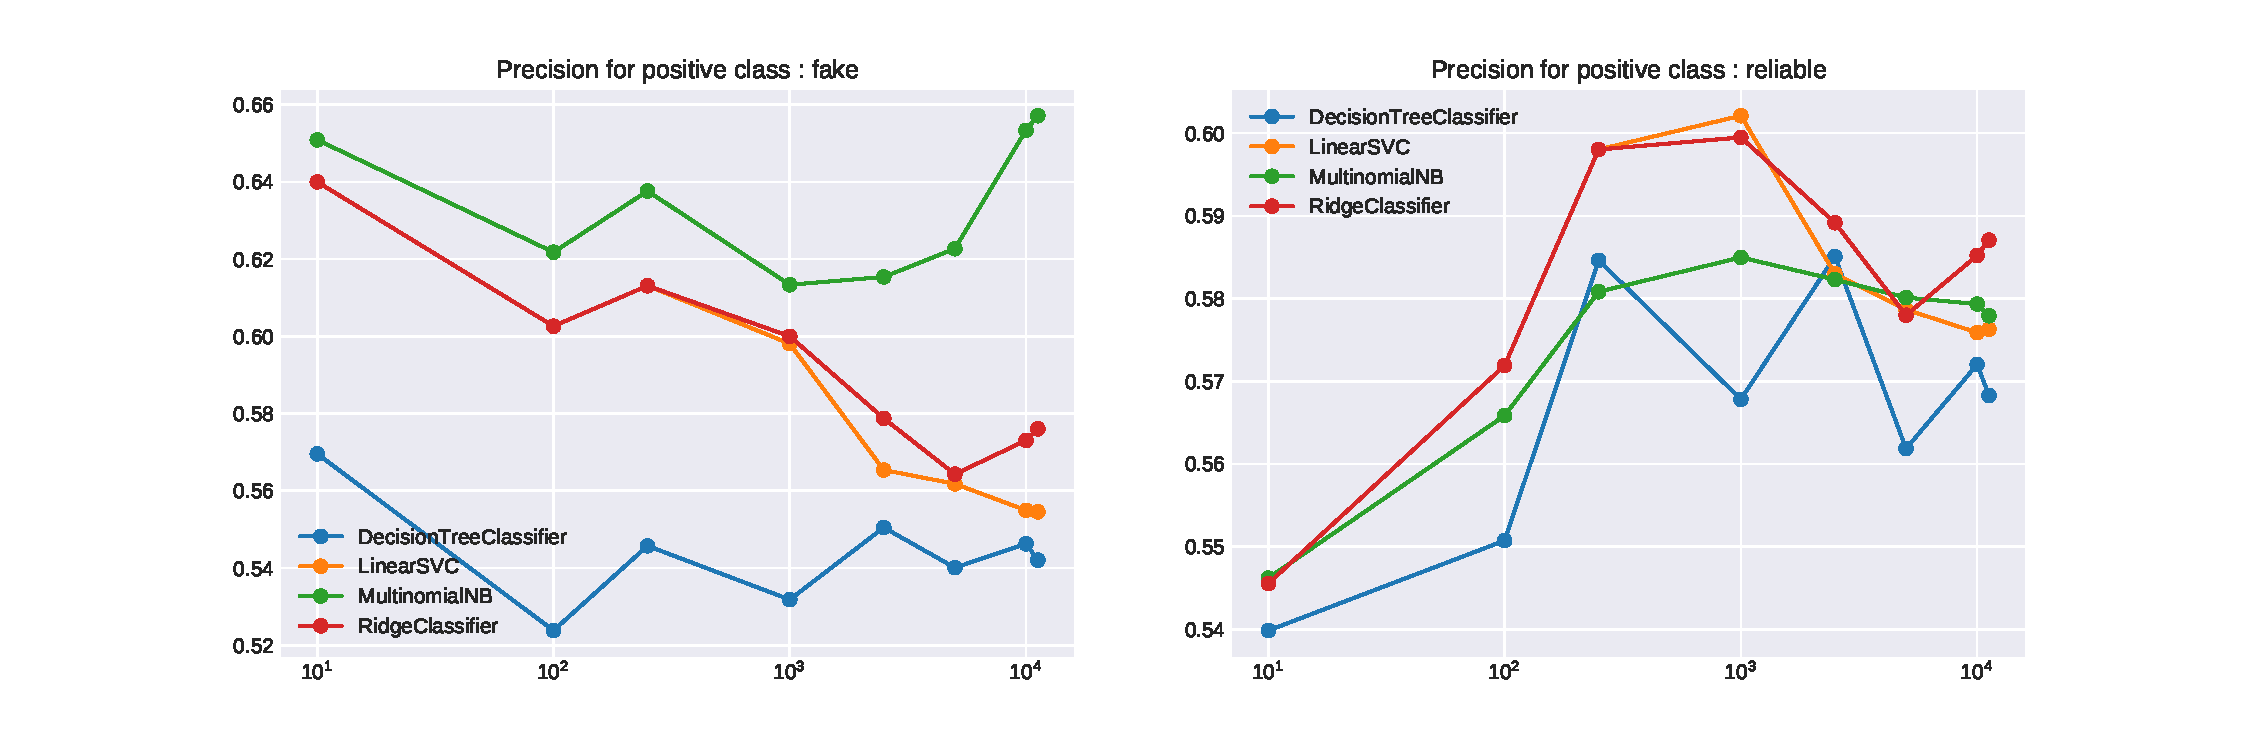
\includegraphics[width=1.2\textwidth]{images/chapitre3/liar-liar_precision_ML}}
	\caption{Precision of the model for each classes, the x axes is log scale of the number of features}
	\label{fig:chap3:max_feature1}
\end{figure*}

\begin{figure*}[h]
	\centering
	\makebox[\textwidth][c]{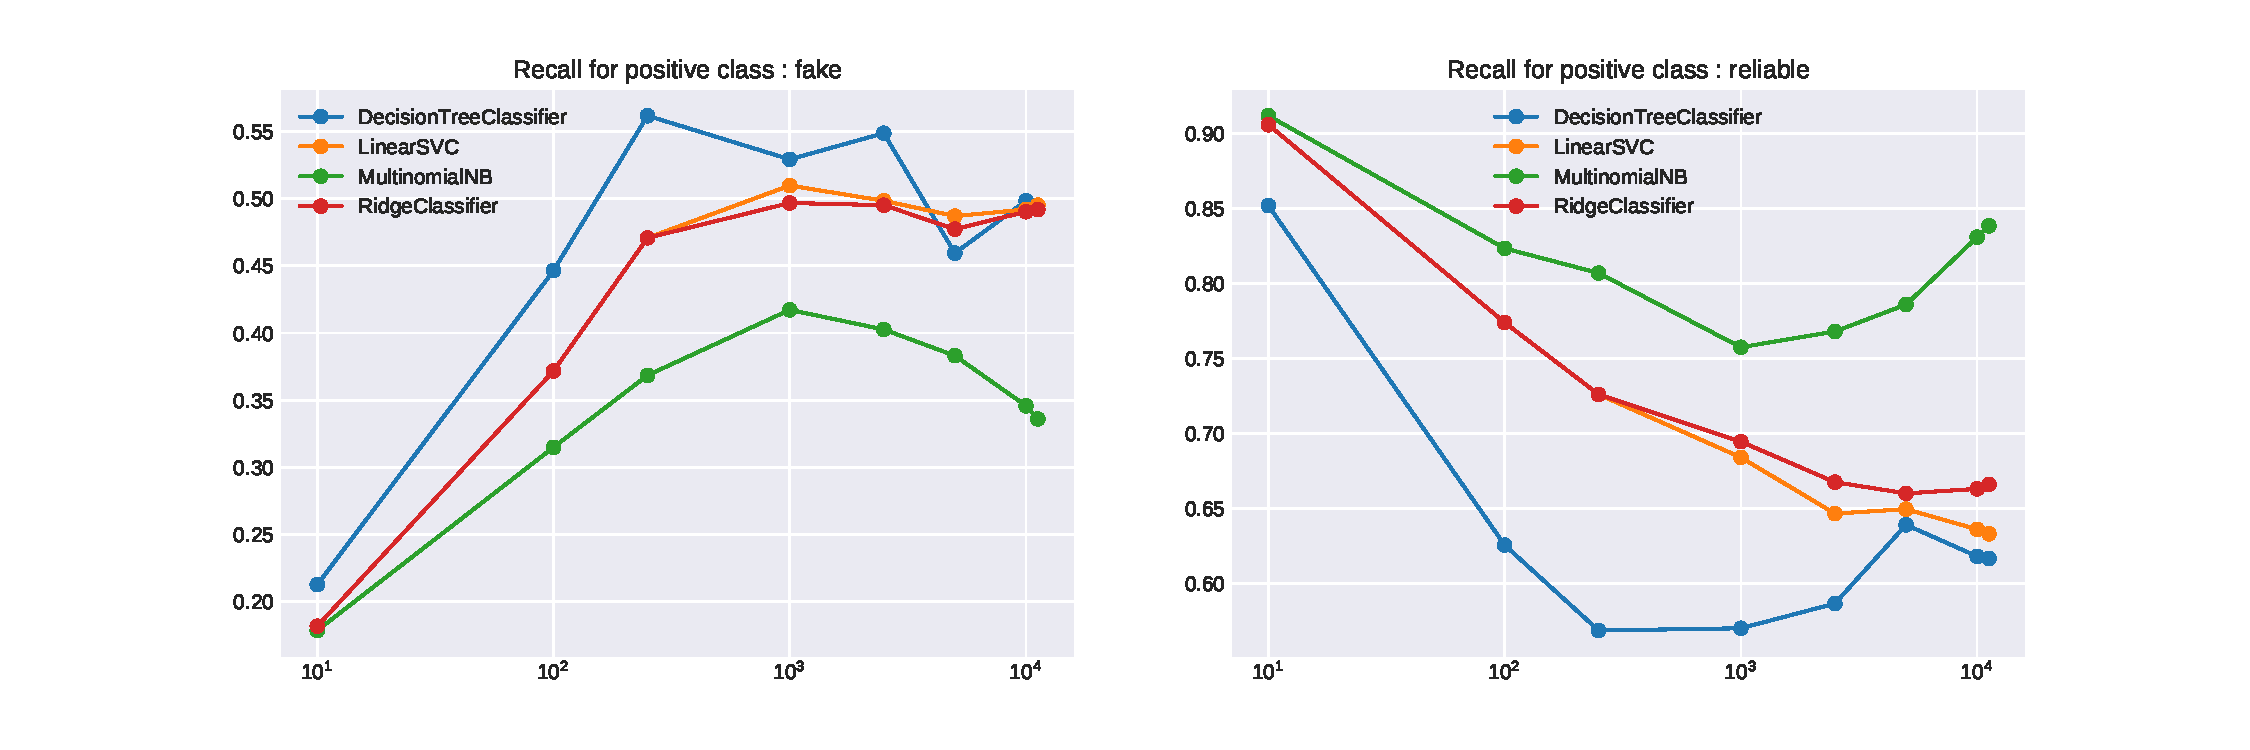
\includegraphics[width=1.2\textwidth]{images/chapitre3/liar-liar_recall_ML}}
	\caption{Precision of the model for each classes, the x axes is log scale of the number of features}
	\label{fig:chap3:max_feature2}
\end{figure*}

\begin{figure*}[h]
	\centering
	\makebox[\textwidth][c]{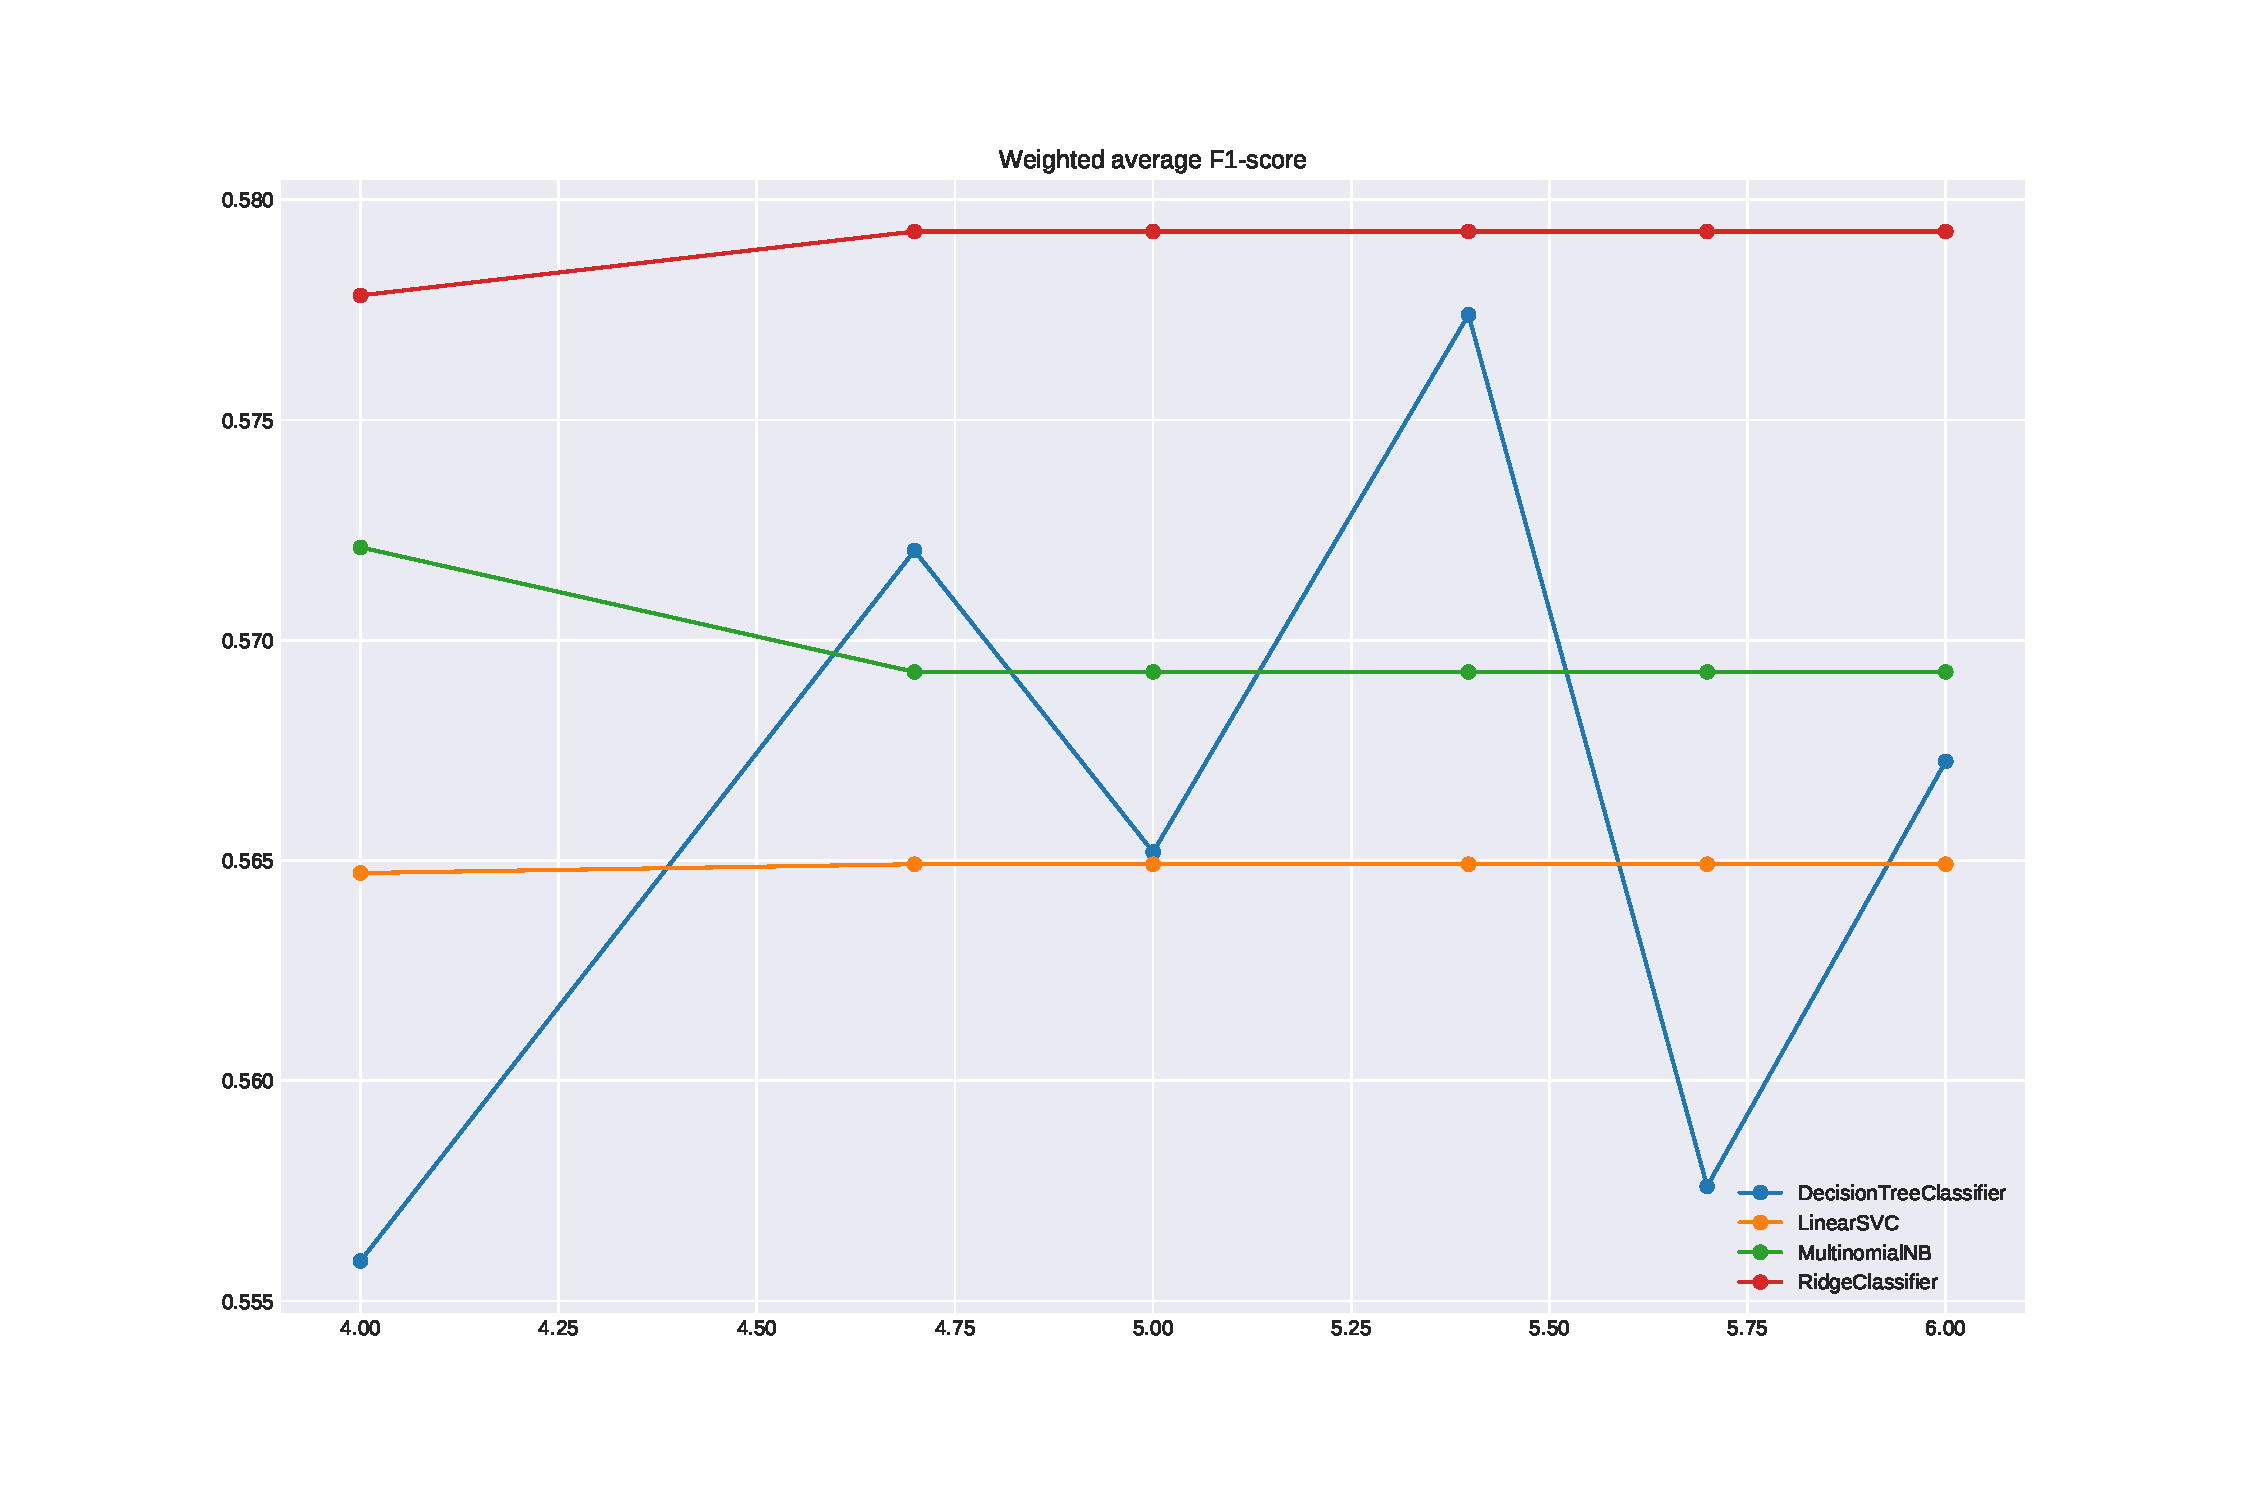
\includegraphics[width=0.8\textwidth]{images/chapitre3/liar-liar_f1_ML}}
	\caption{Precision of the model for each classes, the x axes is log scale of the number of features}
	\label{fig:chap3:max_feature2}
\end{figure*}
\section{Models on fake corpus dataset}